\textbf{\hypertarget{P6}{[\,Suggested Time: 40 mins \textbar \, Total Marks: 20 \textbar \, Challenging\,]}}\\\\
    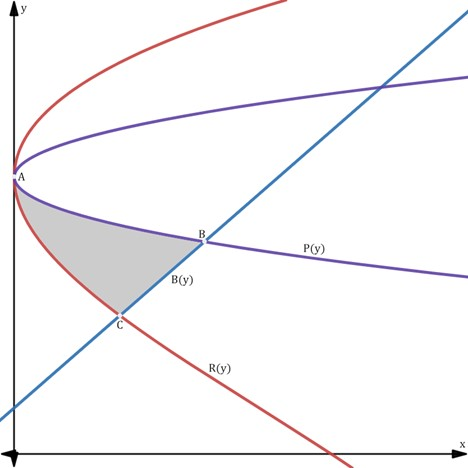
\includegraphics[scale=1]{Question 6 - Graph.jpg}\\
    \textbf{Answers by Accurate drawings or graphical methods are not accepted.}\\
    The graphs are plotting y against x. Point A is a common stationary point of\\
    R(y) and P(y). B(y) passes through the points \(D(10 , 2)\) and \(E(1 , \frac{1}{2})\).\\
    \(P(y) = 28(y - 2)^2\) , \(B(y) = R''(y)\)\\
    Degree of polynomial R(y) is 3.

    \newpage

    Find the shaded area. \textbf{Leave your answers in exact values.} \qnmark{20} \\

%%%%%%%%%%%%%%%%%%
%%%%%Solution%%%%%
%%%%%%%%%%%%%%%%%%

%\newpage \ \newpage \ \newpage \ \newpage

%\begin{comment}

%%%%%Showing that B(y) is linear%%%%%
Degree of \(R(y)\) is 3 \(\implies\) Degree of \(B(y)\) is 1, therefore \(B(y)\) is a linear function \\

%%%%%Finding B(y)%%%%%
Finding the Equation of \(B(y)\)
\begin{align*}
    \displaystyle \text{Gradient} &= \frac{\textstyle \frac{1}{2}-2}{1-10} \\
    \displaystyle          &= \frac{1}{6} \wrkonemark
\end{align*}

\begin{align*}
    \displaystyle   y-2 &= \frac{1}{6}(x-10) \\
    \displaystyle 6y-12 &= x-10 \\
    \displaystyle     x &= 6y-2 \\
    \displaystyle \therefore B(y) &= 6y-2 \wrkonemark \\
\end{align*}

%%%%%Finding R(y) & Point A%%%%%
Finding the coordinates of point A
\begin{equation*}
    \displaystyle P'(y) = 56(y-2)
\end{equation*}
When \(P(y) = 0\)
\begin{align*}
    56(y-2) &= 0 \\
    \therefore y &= 2 \wrkonemark
\end{align*}
Sub \(y = 2\) into \(P(y)\)
\begin{align*}
    \therefore x &= 28(2-2)^{2}\\
                &= 0 \\
    \implies  A &= (0 , 2) \wrkonemark \\
\end{align*}

Finding the equation of \(R(y)\)\\
\textit{Since B(y) = R''(y)}
\begin{align*} %% Finding R'(y)
    \displaystyle R'(y) &= \int{B(y)} \; dy\\
    \displaystyle       &= 3y^{2}-2y+c_{1} , where \; c_{1}\in\mathbb{R} \wrkonemark\\
\end{align*}
Point A is a stationary point of \(R(y) \implies R'(2) = 0\)
\begin{align*} %% Finding c_1
    3(2)^{2}-2(2)+c_{1} &= 0 \\
                  c_{1} &= -8 \wrkonemark \\
    \therefore    R'(y) &= 3y^{2}-2y-8
\end{align*}

\newpage

\begin{align*} %% Integrating R'(y)
    R(y) &= \int{R'(y)} \; dy \\
         &= y^{3}+y^{2}-8y+c_{2} , where \; c_{2}\in\mathbb{R} \wrkonemark
\end{align*}
\textit{When x = 0, y = 2,}
\begin{align*}
                  R(2) &= 0 \\
    2^{3}-2{2}-8+c_{2} &= 0 \\
    \therefore  c_{2} &= 12 \wrkonemark \\
    \implies R(y) &= y^{3}-y^{2}-8y+12 \\
\end{align*}

%%%%%Finding Points B & C%%%%%
Given that Point C is an intercept of \(R(y)\) and \(B(y)\)
\begin{align*} %% Rewriting R(y) =B(y)
    \displaystyle               R(y) &= B(y) \\
    \displaystyle  y^{3}-y^{2}-8y+12 &= 6y-2 \\
    \displaystyle y^{3}-y^{2}-14y+14 &= 0 \wrkonemark
\end{align*}
\begin{align*} %% Solving the equation
    \displaystyle Let \; f(x) &= y^{3}-y^{2}-14y+14 \\
    \displaystyle f(1) &= 0
\end{align*}
\begin{gather*}
    \displaystyle \therefore (y-1) \; \text{is a factor of} \; f(x) \wrkonemark
\end{gather*}
\begin{align*} %% Finding the y-coordinate of C
    \implies f(x) &= (y-1)(y^{2}-14) \\
                  &= 0 \\
\end{align*}

This implies that,
\begin{align*}
    y^{2} &= 14 \\
        y &= \pm\sqrt{14} \\
    \therefore y &= 1 \; or \pm\sqrt{14}
\end{align*}
\begin{gather*}
    Rej. \; y = \pm\sqrt{14} \\
        \implies y = 1 \wrkonemark
\end{gather*}

\begin{align*} %% Finding the x-coordinate of C
    \text{Sub} \; y &= 1 \; \text{into} \; B(y), \\
    B(1) &= 6(1)-2 \\
         &= 4 \\
    \therefore C &= (4,1) \wrkonemark \\
\end{align*}

\newpage

%%%%%Finding Point B%%%%%
Given that Point B is an intercept of P(y) and B(y)
\begin{align*} %% Rewriting the Equation
    \displaystyle 6y-2 &= 28(y-2)^{2} \wrkonemark \\
    \displaystyle      &= 28y^{2}-112y+112
\end{align*}
\begin{align*}
    \displaystyle 2\left(14y^{2}-59y+57\right) &= 0 \\
    \displaystyle               2(7x-19)(2x-3) &= 0 \\
    \displaystyle \therefore y = \frac{19}{7} \; or \; \frac{3}{2}
\end{align*}
Reject \(\displaystyle \; y = \frac{19}{7}\), as it implies that point \(B\) is above \(A\)
\begin{equation*}
    \displaystyle \text{Thus,} \; y = \frac{3}{2} \wrkonemark \\
\end{equation*}

\vspace*{5pt}

Sub \(\displaystyle y = \frac{3}{2}\) into B(y)
\begin{align*} %% Finding Point B
    \displaystyle B\left(\frac{3}{2}\right) &= 6\left(\frac{3}{2}\right)-2 \\
    \displaystyle                           &= 7
\end{align*}
\begin{equation*}
    \displaystyle \therefore B = \left(7,\frac{3}{2}\right) \wrkonemark \\
\end{equation*}

\vspace*{10pt}

%%%%%Finding the shaded area%%%%%
Let \(S\) be the shaded area
\begin{align*}
    \displaystyle S &= \int_{\textstyle \frac{3}{2}}^{2} P(y) \, dy + \frac{1}{2}(4+7)\left(\frac{1}{2}\right) - \int_{1}^{2} R(y) \, dy \\
    \displaystyle   &= \int_{\textstyle \frac{3}{2}}^{2} 28(y-2)^{2} \, dy + \frac{11}{4} - \int_{1}^{2} y^{3}-y^{2}-8y+12 \, dy \wrkonemark \\
    \displaystyle   &= \left[\frac{28}{3}(y-2)^3\right]_{\textstyle \frac{3}{2}}^{2} + \frac{11}{4} - \left[\frac{y^{4}}{4}-\frac{y^{3}}{3}-4y^{2}+12y\right]_{1}^{2} \wrkonemark \\
    \displaystyle   &= \frac{28}{3}(0) - \frac{28}{3}\left(\frac{3}{2}-2\right)^{3} + \frac{11}{4} - \left(\frac{2^{4}}{4} - \frac{2^{3}}{3} - 4(2)^{2} + 12(2) - \left(\frac{1}{4} - \frac{1}{3} - 4 + 12\right)\right) \wrkonemark \\
    \displaystyle   &= \frac{7}{6} + \frac{11}{4} - \frac{17}{12}  \\
    \displaystyle   &= \frac{5}{2} \\
    \\
    \displaystyle   &  \therefore \text{The shaded area is} \; \left(\frac{5}{2}\right) \; units^{2} \ansonemark
\end{align*}

\newpage \ \newpage

%\end{comment}